\section{Introduction}
\label{chap:introduction}
Le filtre de Kalman a été inventé par Rudolf Emil Kálmán en 1960. M. Kálmán était un ingénieur et mathématicien hongrois qui a travaillé sur de nombreux problèmes de filtrage et de contrôle de qualité dans les domaines de l'aérospatiale et de la robotique. Sa théorie des filtres de Kalman est considérée comme l'une des contributions les plus importantes de l'ingénierie moderne et est largement utilisée dans de nombreux domaines pour améliorer la précision de l'estimation des états de systèmes dynamiques.\\

Le filtre de Kalman est un algorithme utilisé pour estimer la valeur d'un système dynamique à partir de mesures soumises à un bruit et incomplètes. Il est souvent utilisé dans les domaines de l'ingénierie, de l'aérospatiale et de la robotique pour améliorer la précision de l'estimation d'un état à un moment donné, en utilisant des mesures précédentes et en prenant en compte le bruit et les erreurs de mesure.

Le filtre de Kalman est basé sur l'hypothèse selon laquelle le système est modélisé par un processus de Markov caché, ce qui signifie que l'état du système à un moment donné ne dépend que de l'état précédent et non des états antérieurs. Le filtre de Kalman utilise des équations de transition de l'état et de mesure pour mettre à jour l'estimation de l'état du système en fonction de nouvelles mesures et de la dynamique du système.\\


Il existe deux variantes du filtre de Kalman : le filtre de Kalman linéaire et le filtre de Kalman non linéaire. Le filtre de Kalman linéaire est utilisé lorsque le système peut être modélisé par des équations linéaires, tandis que le filtre de Kalman non linéaire est utilisé lorsque le système fait alors appel à des fonctions non linéaires.\\

Nous commencerons par une étude approfondie du filtre de Kalman dans sa version Linéaire, puis nous étudierons un cas spécifique du filtre de Kalman étendu.  


\newpage

\section{Filtre de Kalman classique}

\subsection{Présentation théorique du filtre de Kalman}

On pose le modèle d'évolution suivant :

\begin{equation}
	\begin{cases}
		\mathbf{X}_{k} & =\ \mathbf{FX}_{k-1} \ +\ \mathbf{U}_{k}\\
		\mathbf{Y}_{k} & =\ \mathbf{HX}_{k} +\mathbf{V}_{k}
	\end{cases}
\label{eq:1}
\end{equation}	avec dans ce modèle :


\begin{equation}
	\mathbf{X}_{0} \sim \mathcal{N}(\mathbf{m}_{0|0} ,\ \mathbf{P}_{0|0})
\end{equation}
et,
\begin{equation}
	\begin{cases}
		\mathbf{U}_{k} \sim \mathcal{N}(\mathbf{0} ,\ \mathbf{Q})\\
		\mathbf{V}_{k} \sim \mathcal{N}(\mathbf{0} ,\ \mathbf{R})
	\end{cases}
\label{eq:3}
\end{equation}

\notebox{La donnée probabiliste vient de U et V (ce qui implique que X et Y v.a. aussi) mais F, H sont déterministes ! \newline
	On se place ici dans le cadre \textit{linéaire} et \textit{gaussien} les solutions sont donc explicites.
}

D'après \ref{eq:3} et \ref{eq:1} on peut écrire:

\begin{equation}
	\begin{aligned}
		p(\mathbf{X}_{k} |\mathbf{X}_{k-1} =x_{k-1}) & \sim \mathcal{N}(\mathbf{F} x_{k-1} ,\ \mathbf{Q})\\
		p(\mathbf{Y}_{k} |\mathbf{X}_{k} =x_{k}) & \sim \mathcal{N}(\mathbf{H} x_{k} ,\ \mathbf{R})
	\end{aligned}
\label{eq:density}
\end{equation}




Nous cherchons la distribution de $\mathbb{E}(\mathbf{X}_{k} |\mathbf{Y}_{0:k})$ (le meilleur estimateur au sens de l'erreur quadratique moyenne) et, comme le format des équations le fait penser, de façon récursive. \newline 
De plus si la distribution de $p( x_{k} |y_{0:k})$ est normale il suffit de connaitre sa moyenne $\mathbf{m}_{k|k}$ pour avoir $\mathbb{E}(\mathbf{X}_{k} |\mathbf{Y}_{0:k})$.

Nous allons donc montrer que cette distribution est bien normale et qu'il s'agit en réalité d'un problème de propagation des paramètres dans des lois normales puisque que le problème est liée par une relation de récursivité.

On va donc faire l'hypothèse de récurrence suivante : $p( x_{k-1} |y_{0:k-1}) \ \sim \ \mathcal{N}( \mu _{k-1|k-1} ,\ P_{k-1|k-1})$

\notebox{Dans le cadre des développements, nous allons avoir besoin de la propriété suivante :

\begin{equation}
	p( y_{k} |x_{k} ,y_{0:k-1}) =p( y_{k} |x_{k})
	\label{prop:1}
\end{equation}
Nous en faisons une démonstration en annexes  :
}
\newpage

Par ailleurs Bayes nous donne :

\begin{equation}
	\begin{aligned}
		p( x_{k} |y_{0:k}) & =\frac{p( x_{k} ,y_{k} ,y_{0:k-1})}{p( y_{0:k})}\\
		& \\
		& =\frac{p( y_{k} |x_{k} ,y_{0:k-1}) p( x_{k} ,y_{0:k-1})}{\int p( x_{k} ,y_{0:k}) dx_{k}}\\
		& \\
		& =\frac{p( y_{k} |x_{k} ,y_{0:k-1}) p( x_{k} |y_{0:k-1}) p( y_{0:k-1})}{\int p( x_{k} ,y_{0:k}) dx_{k}}\\
		& \\
		& =\frac{p( y_{k} |x_{k} ,y_{0:k-1}) p( x_{k} |y_{0:k-1})\cancel{p( y_{0:k-1})}}{\int p( y_{k} |x_{k} ,y_{0:k-1}) p( x_{k} |y_{0:k-1})\cancel{p( y_{0:k-1})} dx_{k}}
	\end{aligned}
\end{equation}

Et d'après \ref{prop:1} on a finalement,

\begin{equation}
	p( x_{k} |y_{0:k}) =\frac{p( y_{k} |x_{k})\overbrace{p( x_{k} |y_{0:k-1})}^{terme\ de\ prediction}}{\int p( y_{k} |x_{k}) p( x_{k} |y_{0:k-1}) dx_{k}}
\end{equation}


On va procéder par étape et décortiquer ce que cette relation nous permet d'écrire.

On va tout d'abord à exprimer le terme de prédiction comme une loi normale dont on connaitrait les paramètres :

\begin{equation}
	\ \begin{aligned}
		p( x_{k} |y_{0:k-1}) & =\ \int p( x_{k} ,x_{k-1} |y_{0:k-1}) dx_{k-1}\\
		& =\ \int p( x_{k} |x_{k-1}) p( x_{k-1} |y_{0:k-1}) dx_{k-1}\\
		& =\ \int \underbrace{\mathcal{N}(\mathbf{F} x_{k-1} ,\ \mathbf{Q})}_{ p( x_{k} |x_{k-1})}\underbrace{\mathcal{N}( \mu _{k-1|k-1} ,\ \mathbf{P}_{k-1|k-1})}_{Hypothese\ de\ recurence} dx_{k-1}\\
		& =\ \mathcal{N}\left(\mathbf{F} \mu _{k-1|k-1} ,\ \mathbf{Q} +\mathbf{FP}_{k-1|k-1}\mathbf{F}^{T}\right)
	\end{aligned}
\end{equation}

C'est donc notre étape de prédiction, on va passer de \ $\displaystyle \mathbf{X}_{k-1}$à $\displaystyle \mathbf{X}_{k}$ (prédiction) à partir des données $\displaystyle \mathbf{Y}_{0:k-1}$. Cette étape se traduit donc dans la propagation des paramètres d'une loi normale avec la relation de récurrence :

\begin{equation}
	\begin{cases}
		\mu _{k|k-1} \ =\mathbf{F} \mu _{k-1|k-1} \ \\
		\mathbf{P}_{k|k-1} =\mathbf{Q} +\mathbf{FP}_{k-1|k-1}\mathbf{F}^{T}
	\end{cases}
\end{equation}


L'étape de prédiction faite on cherche maintenant à intégrer la nouvelle observation, c'est à dire calculer notre terme : $\displaystyle p( x_{k} |y_{0:k})$.


\newpage


On va donc réaliser l'étape de filtrage (ou étape d'update) :

Nous auront pour cela, besoin d'un résultat :

\begin{Theorem}{}{Loi normale}
	\begin{equation*}
		\mathcal{N}( y|\mathbf{H} x,\ \mathbf{R})\mathcal{N}( x|\mathbf{m} ,\ \mathbf{P}) \ =\ q( y)\mathcal{N}( x|\hat{\mathbf{m}} ,\ \hat{\mathbf{P}})
	\end{equation*}
Avec,
	\begin{gather*}
		\hat{\mathbf{m}} \ =\ \mathbf{m} \ +\ \mathbf{K}( y-\mathbf{Hm})\\
		\hat{\mathbf{P}} =(\mathbf{I} -\mathbf{KH})\mathbf{P}\\
		\mathbf{K} =\mathbf{PH}^{T}\left(\mathbf{HPH}^{T} +\mathbf{R}\right)^{-1}
	\end{gather*}
\end{Theorem}

Cette propriété et  \ref{eq:density} nous permet d'écrire:

\begin{equation}
	\begin{aligned}
		p( x_{k} |y_{0:k}) & =\frac{p( y_{k} |x_{k}) p( x_{k} |y_{0:k-1})}{\int p( y_{k} |x_{k}) p( x_{k} |y_{0:k-1}) dx_{k}}\\
		& \\
		& \propto \frac{g( y_{k})\mathcal{N}( x_{k} |\mu _{k|k} ,\ \mathbf{P}_{k|k})}{\int g( y_{k})\mathcal{N}( x_{k} |\mu _{k|k} ,\ \mathbf{P}_{k|k}) dx_{k}}
	\end{aligned} \ 
\end{equation}


or ici,

\begin{equation}
	\frac{g( y_{k})\mathcal{N}( x_{k} |\mu _{k|k} ,\ \mathbf{P}_{k|k})}{\int g( y_{k})\mathcal{N}( x_{k} |\mu _{k|k} ,\ \mathbf{P}_{k|k}) dx_{k}} =\frac{\cancel{g( y_{k})}\mathcal{N}( x_{k} |\mu _{k|k} ,\ \mathbf{P}_{k|k})}{\cancel{g( y_{k})}\int \mathcal{N}( x_{k} |\mu _{k|k} ,\ \mathbf{P}_{k|k}) dx_{k}}
\end{equation}


Et, comme on marginalise par rapport à $\displaystyle x_{k}$, $\int \mathcal{N}( x_{k} |\mu _{k|k} ,\ \mathbf{P}_{k|k}) dx_{k} = 1$ on obtient donc finalement :


\begin{equation*}
	p( x_{k} |y_{0:k}) \ \propto \mathcal{N}( x_{k} |\mu _{k|k} ,\ \mathbf{P}_{k|k})
\end{equation*}
avec :


\begin{equation}
	\begin{cases}
		\mu _{k|k} =\mu _{k|k-1} \ +\ \mathbf{K}( y_{k} -\mathbf{H} \mu _{k|k-1})\\
		\mathbf{P}_{k|k} =(\mathbf{I} -\mathbf{KH})\mathbf{P}_{k|k-1}\\
		\mathbf{K} =\mathbf{P_{k|k-1} H}^{T}\left(\mathbf{HP_{k|k-1} H}^{T} +\mathbf{R}\right)^{-1}
	\end{cases}
\label{eq:end}
\end{equation}
\newpage
On peut résumer nos différentes étapes par ce schémas:
\newline
\\
\\
	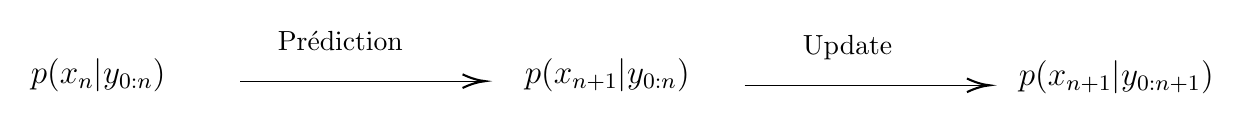
\begin{tikzpicture}[x=0.75pt,y=0.75pt,yscale=-1,xscale=1]
		%uncomment if require: \path (0,120); %set diagram left start at 0, and has height of 120
		%Straight Lines [id:da21205328503481824] 
		\draw    (153.2,88.5) -- (269.2,88.5) ;
		\draw [shift={(271.2,88.5)}, rotate = 180] [color={rgb, 255:red, 0; green, 0; blue, 0 }  ][line width=0.75]    (10.93,-3.29) .. controls (6.95,-1.4) and (3.31,-0.3) .. (0,0) .. controls (3.31,0.3) and (6.95,1.4) .. (10.93,3.29)   ;
		%Straight Lines [id:da08941471988106997] 
		\draw    (396.2,90.5) -- (512.2,90.5) ;
		\draw [shift={(514.2,90.5)}, rotate = 180] [color={rgb, 255:red, 0; green, 0; blue, 0 }  ][line width=0.75]    (10.93,-3.29) .. controls (6.95,-1.4) and (3.31,-0.3) .. (0,0) .. controls (3.31,0.3) and (6.95,1.4) .. (10.93,3.29)   ;
		
		% Text Node
		\draw (51,76.4) node [anchor=north west][inner sep=0.75pt]  [font=\large]  {$p( x_{n} |y_{0:n})$};
		% Text Node
		\draw (289,76.4) node [anchor=north west][inner sep=0.75pt]  [font=\large]  {$p( x_{n+1} |y_{0:n})$};
		% Text Node
		\draw (527,77.4) node [anchor=north west][inner sep=0.75pt]  [font=\large]  {$p( x_{n+1} |y_{0:n+1})$};
		% Text Node
		\draw (170,63) node [anchor=north west][inner sep=0.75pt]   [align=left] {Prédiction};
		% Text Node
		\draw (423,65) node [anchor=north west][inner sep=0.75pt]   [align=left] {Update};	
	\end{tikzpicture}

Nous allons donc maintenant nous atteler à l'implémentation d'un filtre de Kalman simple. 



\subsection{Implémentation}

Une expression générale intégrale possible de la position est la suivante: $\displaystyle x( t) \ =\ x( t') \ +\ \int _{t'}^{t} v( \tau ) d\tau $. En discrétisant $\displaystyle \frac{dx( t)}{dt} =v( t)$ on obtient $\displaystyle x_{n+1} \approx x_{n} +v\times dt$.



Avec une démarche similaire pour les ordonées et en supposant une vitesse constante nous obtenons:


\begin{equation}
	\mathbf{X}_{n+1} =\begin{bmatrix}
		1 & dt & 0 & 0\\
		0 & 1 & 0 & 0\\
		0 & 0 & 1 & dt\\
		0 & 0 & 0 & 1
	\end{bmatrix} \times \mathbf{X}_{n}
\end{equation}


Rappel, ici : $\displaystyle X\ =\ [ x,\ \dot{x} ,y,\dot{y}]^{T}$



De même, en supposant que les mesures contiennent la "vraie" position plus un bruit d'erreur:


\begin{equation}
	\mathbf{Y}_{n+1} =\begin{bmatrix}
		1 & 0 & 0 & 0\\
		0 & 0 & 1 & 0
	\end{bmatrix} \times \mathbf{X}_{n+1} +v_{n+1}
\end{equation}
En ajoutant dans la première équation un bruit représentant la confiance en ce modèle (vitesse constante) nous obtenons les mêmes expressions que celles énoncées dans la partie précédente. En supposant que le vecteur d'état initial est gaussien et que les bruits de ce modèle sont gaussiens on peut alors appliquer les résutats du Filtre de Kalman !



\textit{On remarque ici que H et F sont constantes (ne dépendent pas je n) nous sommes dans le cas simplifié de chaînes homogènes !}

Nous allons procéder en 3 étapes pour l'implémentation du filtre de Kalman sur notre exemple de TP. \newline
Dans une première partie nous présenterons notre initialisation avec la création de la trajectoire théorique, des observations et des différents paramètres nécessaires et les conséquences de leur modification. \newline
Dans une seconde partie, nous verrons comment implémenter le cœur du filtre et quelques conditions à respecter. \newline
Finalement nous verrons l'implémentation d'une métrique d'erreur et des résultats finaux !


\newpage

\subsubsection{Initialisation}

On va créer nos observations et notre trajectoire à partir du modèle décrit ci-dessus, on va donc écrire le code python suivant :

\begin{lstlisting}[language=Python, caption=Initialisation du filter]
def creer_trajectoire(F, Q, x_init, T):
		vecteur_x = np.zeros((4, T))
		vecteur_x[:, 0] = x_init
		for i in range(1, len(vecteur_x[0])):
			vecteur_x[:, i] = F@vecteur_x[:, i-1] + \
			np.random.multivariate_normal(np.zeros((4)), Q)
		return vecteur_x

def creer_observations(H, R, vecteur_x, T):
		vecteur_y = np.zeros((2, T))
		for i in range(0, len(vecteur_y[0])):
			vecteur_y[:, i] = H@vecteur_x[:, i] + \
			np.random.multivariate_normal(np.zeros(2), R)
		return vecteur_y
\end{lstlisting}

Avec les matrices $\mathbf{Q}, \mathbf{F}, \mathbf{H}, \mathbf{R}, \mathbf{T}$ données dans l'énoncé et rappelées plus haut.

On obtient alors les exemples de trajectoires et d'observations suivantes:


\begin{figure}[hbt!]
	\centering
	\includegraphics[scale=0.3]{./images/init.png}
	\caption{\centering exemple de trajectoire et observations simulées}
	\label{fig:init_out}
\end{figure}
\FloatBarrier

Lorsque le bruit du modèle est faible (fig (1, 1), (1, 2)) on observe une trajectoire relativement proche d'une droite (ce qui est cohérent vis à vis d'une vitesse constante).\\
En revanche la trajectoire réelle devient rapidement et fortement non linéaire lorsque $sigma_{Q}$ augment (2e et 3e ligne). \\
De manière générale l'importance de la dispersion des observations autour de la vraie courbe corrèle bien avec l'augmentation du bruit de mesure et la complexité de la trajectoire semble bien répondre à une augmentation de $sigma_{Q}$ (forte variation de la vitesse réelle).\\
On peut donc considérer notre problème initié, il ne reste plus qu'a faire l'implémentation du filtre à proprement parlé.\\
Avant de passer à son implémentation en code il nous faut considérer les conditions initiales suivantes :

\begin{equation*}
	\begin{cases}
		Accele ration\ :\ a_{0} =0\\
		Vitesse:\ v_{0}^{x} ,\ v_{0}^{y} \ =\ [ 40,\ 20]\\
		Position\ :\ [ x_{0} ,y_{0}] \ =\ [ 3,\ -4]
	\end{cases}
\end{equation*}

On va par ailleurs initialiser $Q$ et $R$ comme donnée dans l'énoncé (voir code...), de même pour $\mathbf{X}_{0}$ : on va choisir une matrice de covariance $\mathbf{P}_{0|0}$ "faible" si la position de départ est bien connue et inversement si grande incertitude.\\
On a alors le code python suivant:
\begin{lstlisting}[language=Python, caption=Fonction de calcul du filtre de kalman à l'instant k]
T_e = 1
T = 100
sigma_Q = 1
sigma_px = 30
sigma_py = 30

F = np.eye(4)
F[0, 1], F[2, 3] = T_e, T_e
Q = np.array([
[T_e**3/3, T_e**2/2, 0, 0],
[T_e**2/2, T_e, 0, 0],
[0, 0, T_e**3/3, T_e**2/2],
[0, 0, T_e**2/2, T_e]], dtype='float64'
)*sigma_Q**2

H = np.zeros((2, 4))
H[0, 0], H[1, 2] = 1, 1
R = np.diag([sigma_px**2, sigma_py**2])

x_init = np.array([3, 40, -4, 20])

x_kalm = x_init  # x^_0|0
P_kalm = np.eye(4)  # P_0|0
\end{lstlisting}

On ne mets ici que des extraits du code, le code complet est disponible en annexe.

\newpage

\subsubsection{Implémentation du filtre de Kalman simple}

Nous allons donc reprendre les équations décrites en \ref{eq:end} et les implémenter en python, on obtient alors:
\begin{lstlisting}[language=Python, caption=Fonction de calcul du filtre de kalman à l'instant k]
		def filtre_de_kalman(F, Q, H, R, y_k, x_kalm_prec, P_kalm_prec):
		
		# prediction :
		m_prediction = F@x_kalm_prec
		P_prediction = Q + F@P_kalm_prec@F.T
		
		# update
		K = P_prediction@H.T@np.linalg.inv(H@P_prediction@H.T + R)
		# Mise a jour des vecteurs
		x_kalm_k = m_prediction + K@(y_k - H@m_prediction)
		P_kalm_k = (np.eye(len(P_kalm_prec[0])) - K@H)@P_prediction
		
		# Return a l'etape k des vecteurs
		return [x_kalm_k, P_kalm_k]
\end{lstlisting}

Cette fonction nous permet de faire nos étape d'update et de prédiction récursivement sur les données qui arrivent, on peut alors écrire le programme dans sa globalité qui va utiliser les observations générées et garder en mémoire nos prédictions pour un affichage ultérieur :

\begin{lstlisting}[language=Python, caption=Fonction principale filtre de kalman simple]
	vecteur_x = creer_trajectoire(F, Q, x_init, T)
	vecteur_y = creer_observations(H, R, vecteur_x, T)
	
	# Initialisation des differentes variables
	# ....
	
	# Estimation des etats
	for i in range(1,T):
	x_est[:,i],  P_est[:, :,i] = filtre_de_kalman(F, Q, H, R, vecteur_y[:,i], x_est[:,i-1], P_est[:, :,i-1])
\end{lstlisting}

\warningbox{Ici les codes sont allégés pour une meilleure compréhension des étapes clés. Le code complet est disponible en annexe \ref{code_source} (projet github)}

\notebox{On se muni également d'une fonction nous permettant de calculer l'erreur quadratique entre notre estimation et nos valeurs réelles sur l'ensemble de nos prédictions (voir source code) : \textit{erreur\_quad(x\_est, vecteur\_x) }
}

\newpage

\subsubsection{Les résultats}

Une fois notre implémentation réalisé, nous allons jouer sur les paramètre du modèle, ici :
\begin{itemize}
	\item $\sigma_{Q}$ nous donne la confiance du modèle : nous allons le faire varier de 1 (grande confiance) à 10 (confiance très faible)
	\item $\sigma_{px}$ et $\sigma_{py}$ représentent le bruit d'observation (nos erreurs d'observation) que nous allons faire varier de 10 (faible bruit) à 300 (très fort bruit)
\end{itemize}


On obtient comme courbe de référence (confiance forte et faible bruit ) :

\begin{figure}[hbt!]
	\centering
	\includegraphics[scale=0.5]{./images/res1.png}
	\caption{\centering Résultat du filtre de Kalman Simple, courbe en vert : notre estimation}
\end{figure}
\FloatBarrier

\newpage

Si on réduit notre confiance sur le modèle (on augmente Q) on obtient alors :

\begin{figure}[hbt!]
	\centering
	\includegraphics[scale=0.4]{./images/res2.png}
	\caption{\centering Résultat du filtre de Kalman Simple, courbe en vert : notre estimation}
\end{figure}
\FloatBarrier

Puis pour une version dégradé ($\sigma_{Q} = 10 $),


\begin{figure}[hbt!]
	\centering
	\includegraphics[scale=0.4]{./images/res3.png}
	\caption{\centering Résultat du filtre de Kalman Simple, courbe en vert : notre estimation}
\end{figure}
\FloatBarrier
On continue l'expérience avec les autres valeurs comme annoncé plus haut.
\newpage
On obtient alors de la même façon :
\begin{figure}[hbt!]
	\centering
	\includegraphics[scale=1]{./images/rr.png}
	\caption{\centering Résultats du filtre de Kalman Simple, avec différentes valeurs de bruit}
\end{figure}
\FloatBarrier

Nous analysons les résultats sur la prochaine page...

\newpage

Il semblerait que pour des erreurs de mesures ($\sigma_{px}$ et $\sigma_{py}$) faibles le filtre reste capable de suivre le mouvement en dépit de variations importantes de $\sigma_{Q}$. Cependant nous observons dors et déjà les limites du Filtre de Kalman : si dans les cas de
grande confiance dans notre modèle (fig (1,1), 2) l’approximation est bonne malgré des bruits de mesure qui peuvent être conséquents, il ne l’est absolument plus dès que les deux bruits augmentent simultanément. En effet lorsqu'une information est mauvaise le filtre à tendance à s’appuyer sur l’autre pour prédire, mais si les deux sont imprécises les erreurs se cumulent et l’algorithme devient rapidement peu performant (fig (3, 2)).

\newpage

\section{Filtre de Kalman étendu}

\subsection{Introduction}
Certains phénomènes de suivi n’admettent pas une modélisation linéaire de la forme :

\begin{equation}
	\begin{cases}
		\hline
		\mathbf{X}_{k} & =\ \mathbf{FX}_{k-1} \ +\ \mathbf{U}_{k}\\
		\mathbf{Y}_{k} & =\ \mathbf{HX}_{k} +\mathbf{V}_{k}
	\end{cases}
\end{equation}

mais une forme plus générale qui peut être exprimée comme :

\begin{equation}
	\begin{cases}
		\hline
		\mathbf{X}_{k} & =\ f(\mathbf{X}_{k-1})\\
		\mathbf{Y}_{k} & =\ g(\mathbf{X}_{k})
	\end{cases}
\end{equation}
avec $\displaystyle f$ et $\displaystyle g$ de $\displaystyle \Re ^{d}$ dans $\displaystyle \Re ^{d}$.
\newline
Or si ces fonctions présentent des non-linéarités les résultats explicites du filtre (exprimés partie
1 : \ref{eq:end}) ne sont plus valables. Pour palier ce problème une solution est de changer d’algorithme, d’en choisir un plus contraignant en terme de puissance de calcul mais capable de suivre ce type de phénomène. Nous pourrions par exemple nommer celui du filtrage particulaire. Une autre est d’essayer de se ramener à une situation linéaire où nous pourrons à nouveau utiliser les résultats du filtre. C’est l’approche que propose de réaliser cette partie

\subsection{Formulation du problème}

Dans notre cas nous considérons le passage en coordonnées sphérique pour les observation.
On prendra dans la suite ce référentiel :\\
	\begin{figure}[hbt!]
		\centering
		\begin{tikzpicture}[x=0.75pt,y=0.75pt,yscale=-1,xscale=1]
			%uncomment if require: \path (0,171); %set diagram left start at 0, and has height of 171
			
			%Straight Lines [id:da49847039920212244] 
			\draw    (283.33,146.2) -- (283.33,17.53) ;
			\draw [shift={(283.33,15.53)}, rotate = 90] [color={rgb, 255:red, 0; green, 0; blue, 0 }  ][line width=0.75]    (10.93,-3.29) .. controls (6.95,-1.4) and (3.31,-0.3) .. (0,0) .. controls (3.31,0.3) and (6.95,1.4) .. (10.93,3.29)   ;
			%Straight Lines [id:da5650431273973175] 
			\draw    (283.33,146.2) -- (419.4,146.2) ;
			\draw [shift={(421.4,146.2)}, rotate = 180] [color={rgb, 255:red, 0; green, 0; blue, 0 }  ][line width=0.75]    (10.93,-3.29) .. controls (6.95,-1.4) and (3.31,-0.3) .. (0,0) .. controls (3.31,0.3) and (6.95,1.4) .. (10.93,3.29)   ;
			%Straight Lines [id:da4768522786600511] 
			\draw    (283.33,146.2) -- (373.4,58.2) ;
			%Straight Lines [id:da6045611475887867] 
			\draw  [dash pattern={on 0.84pt off 2.51pt}]  (373.4,58.2) -- (373.4,146.2) ;
			%Straight Lines [id:da40488962930943817] 
			\draw  [dash pattern={on 0.84pt off 2.51pt}]  (373.4,58.2) -- (282.73,58.2) ;
			%Curve Lines [id:da7610675001237099] 
			\draw    (314.07,145.53) .. controls (319.62,135.05) and (312.05,130.84) .. (305.6,126.05) ;
			\draw [shift={(304.07,124.87)}, rotate = 38.66] [color={rgb, 255:red, 0; green, 0; blue, 0 }  ][line width=0.75]    (10.93,-3.29) .. controls (6.95,-1.4) and (3.31,-0.3) .. (0,0) .. controls (3.31,0.3) and (6.95,1.4) .. (10.93,3.29)   ;
			
			% Text Node
			\draw (320.67,127.73) node [anchor=north west][inner sep=0.75pt]  [font=\scriptsize]  {$\theta $};
			% Text Node
			\draw (311.33,91.07) node [anchor=north west][inner sep=0.75pt]    {$r$};
			% Text Node
			\draw (266,7.4) node [anchor=north west][inner sep=0.75pt]    {$y$};
			% Text Node
			\draw (418,144.4) node [anchor=north west][inner sep=0.75pt]    {$x$};
			% Text Node
			\draw (260,49.07) node [anchor=north west][inner sep=0.75pt]    {$p_{y}$};
			% Text Node
			\draw (369,146.07) node [anchor=north west][inner sep=0.75pt]    {$p_{x}$};
		\end{tikzpicture}
	\end{figure}


On va donc représenter nos nouvelles variables, en commencent par notre variable d'état qui ne change pas :
\begin{equation}
	\mathbf{X} =\begin{bmatrix}
		p_{x}\\
		v_{x}\\
		p_{y}\\
		v_{y}
	\end{bmatrix}
\end{equation}

Puis notre variable d'observation qui passe en polaire :
\begin{equation}
	\mathbf{Y} =\begin{bmatrix}
		p_{x}\\
		p_{y}
	\end{bmatrix}\xrightarrow{Polaire}\begin{bmatrix}
		\theta \\
		r
	\end{bmatrix}
\end{equation}

On peut alors faire le changement de référentiel à l'aide de :

\begin{equation}
	\begin{cases}
		\theta ( p_{x} ,p_{y}) =\arctan\left(\frac{p_{y}}{p_{x}}\right)\\
		\\\\
		r( p_{x} ,p_{y}) =\sqrt{p_{x}^{2} +p_{y}^{2}}
	\end{cases}
\end{equation}

Ce qui nous donne pour la variable d'observation :


\begin{equation}
	\begin{aligned}
		\mathbf{Y}_{k} & & =\begin{bmatrix}
			\theta (\mathbf{X}_{k})\\
			r(\mathbf{X}_{k})
		\end{bmatrix} +V_{k}\\
		& & \\
		& & =g(\mathbf{X}_{k})
	\end{aligned}
\end{equation}
avec $\displaystyle v_{k} \sim \mathcal{N}( 0,\mathbf{R})$

\warningbox{Attention, ici g est \textbf{non linéaire} (par le arctan et la racine)}

On cherche donc à linéariser $g$, on dispose pour cela de Taylor-Lagrange qui nous dit :
Pour toute fonction de $\displaystyle \mathcal{C}^{1}$ de $\displaystyle \Re ^{d}$ dans $\displaystyle \Re ^{m}$ on peut écrire :

\begin{equation}
	f( x) \approx f( x_{0}) +J( f)( x_{0})( x-x_{0})
\end{equation}
avec $\displaystyle J$ la jacobienne de $\displaystyle f$.

Un rapide calcul nous donne dans notre cas :

\begin{equation}
	\mathbf{J}_{g} =\frac{\partial g}{\partial \mathbf{X}}\Bigl|_{\mathbf{X}_{k} =\mu _{k|k-1}} =\begin{bmatrix}
		-\frac{p_{y}}{p_{x}^{2} +p_{y}^{2}} & 0 & \frac{p_{x}}{p_{x}^{2} +p_{y}^{2}} & 0\\
		\frac{p_{x}}{\sqrt{p_{x}^{2} +p_{y}^{2}}} & 0 & \frac{p_{y}}{\sqrt{p_{x}^{2} +p_{y}^{2}}} & 0
	\end{bmatrix}
\end{equation}

Ce qui nous permet d'écrire d'après Tailor Lagrange autour de $\displaystyle \mu _{k|k-1}$,

\begin{equation}
	\mathbf{Y}_{k} \approx g( \mu _{k|k-1}) +\mathbf{J}_{g}( \mu _{k|k-1}) \times (\mathbf{X}_{k} -\mu _{k|k-1}) +V_{k}
\end{equation}

En réarrangeant les termes pour faire apparaitre une écriture sous la forme (\ref{eq:1}), on peut écrire :
\begin{equation}
	\mathbf{Y}_{k} \approx \mathbf{J}_{g}( \mu _{k|k-1})\mathbf{X}_{k} +\underbrace{g( \mu _{k|k-1}) -\mathbf{J}_{g}( \mu _{k|k-1}) \mu _{k|k-1} +V_{k}}_{r_{k} ,\ Biais\ introduit\ par\ la\ linearisation}
\end{equation}

Comme on cherche un modèle du type $\displaystyle y_{k} =H( \mu _{k|k-1}) X_{k} + V_{k}$ on va implémenter:

\begin{equation}
	\underbrace{\widetilde{y_{k}}}_{ \begin{array}{l}
			Ce\ que\ l'on\ va\ \\
			implementer\ dans\ le\ code
	\end{array}} =y_{k} -g( \mu _{k|k-1}) +\mathbf{J}_{g}( \mu _{k|k-1}) \mu _{k|k-1}
\end{equation}

\subsection{Implémentation}

Avec notre modélisation du problème ci-dessus, l'implémentation est assez simple, on reprends le code de la partie 1 (filtre Kalman simple) en y apportant quelques modifications pour prendre en compte notre linéarisation.\\
\\
Pour se faire on va commencer par implémenter le calcul de la jacobienne :
\begin{lstlisting}[language=Python, caption=Fonction de calcul de la jacobienne de g]
	def evaluate_jacobian(mu):
		# last prediction format : [p_x, v_x, p_y, v_y]
		return np.array([
		[(-mu[2])/(mu[0]**2 + mu[2]**2), 0, mu[0]/(mu[0]**2 + mu[2]**2), 0],
		[mu[0]/np.sqrt(mu[0]**2 + mu[2]**2), 0, mu[2] /
		np.sqrt(mu[0]**2 + mu[2]**2), 0]
		])
\end{lstlisting}

Puis on va directement remplacer l'ancienne fonction de calcul d'étape du filtre de Kalman en remplaçant :


\begin{equation}
	\begin{cases}
		\mathbf{H} =\mathbf{J}_{g}\left(\underbrace{\mu _{k|k-1}}_{prediction\ que\ l'on\ utilise\ comme\ la\ meilleur\ approximation\ de\ X}\right)\\
		\\\\
		y_{k_{EKF}} =y_{k} -g( \mu _{k|k-1}) +\mathbf{J}_{g}( \mu _{k|k-1}) \mu _{k|k-1}
	\end{cases}
\end{equation}
\newpage
Ce qui donne en python :
\begin{lstlisting}[language=Python, caption=Filtre de Kalman Etendu]
	def filtre_de_kalman_extended(F, Q, R, y_k, x_kalm_prec, P_kalm_prec):
			# prediction :
			mu_prediction = F@x_kalm_prec
			# On va utiliser m_prediction comme meilleure approximation de X
			# a l'instant k !
			P_prediction = Q + F@P_kalm_prec@F.T
			
			# Variables upadte pour l'update de l'EKF:
			y_k_new = y_k - g(mu_prediction) + \
			evaluate_jacobian(mu_prediction)@mu_prediction
			# La nouvelle matrice H issue de la linearisation:
			H = evaluate_jacobian(mu_prediction)
			
			# update
			K = P_prediction@H.T@np.linalg.inv(H@P_prediction@H.T + R)
			# Mise a jour des vecteurs
			x_kalm_k = mu_prediction + K@(y_k_new - H@mu_prediction)
			P_kalm_k = (np.eye(len(P_kalm_prec[0])) - K@H)@P_prediction
			
			# Return a l'etape k des vecteurs
			return [x_kalm_k, P_kalm_k]
\end{lstlisting}

Avant de passer aux résultats, il est important de noter que nos observations sont donc dans le format de coordonnées polaire, pour faire l'affichage sous forme de graph il faut donc les retransformer dans le système cartésien, ce que l'on fait dans le programme principal qui lui ne change pas par rapport à la première version :
\begin{lstlisting}[language=Python, caption=Filtre de Kalman Etendu]
# Meme exercice mais avec l'EKF:
vecteur_x = creer_trajectoire(F, Q, x_init, T)
vecteur_y = creer_observation_EKF(R_EKF, vecteur_x, T)

# Estimation des etats
#.... 


# On fait la transformation inverse pour l'affichage des donnees observees en cartesien:
vecteur_y_converted = np.zeros((2,100))
for i in range(T):
vecteur_y_converted[0, i] = vecteur_y[1, i]*np.cos(vecteur_y[0, i])
vecteur_y_converted[1, i] = vecteur_y[1, i]*np.sin(vecteur_y[0, i])

# Plot the data:
draw_all2(vecteur_x, vecteur_y_converted, x_est, sigma_Q, sigma_px, sigma_py, erreur_quad(x_est, vecteur_x))
\end{lstlisting}

On peut donc maintenant passer aux résultats.

\subsection{Résultats}
On va procéder comme pour la partie 1. On simule avec les même valeurs de $\sigma_{Q}$ et de $\sigma_{px}$, $\sigma_{py}$.\\
On obtient alors :
\begin{figure}[hbt!]
	\centering
	\includegraphics[scale=1]{./images/ee.png}
	\caption{\centering Résultats du filtre de Kalman étendu, avec différentes valeurs de bruit}
\end{figure}
\FloatBarrier

On peut faire plusieurs remarques :\\
L'évolution du comportement de notre filtre avec nos différents niveaux de bruits semble correspondre à ce que l'on a obtenu dans la première partie. A la différence qu'il semble perdre en qualité au fur et à mesure que l'on augmente le nombre d'observation, on s'en rend bien compte en fin de nos trajectoires la prédiction commence à être bruité. Cela peut avoir comme origine la propagation du biais liée à notre linéarisation. Il dépend de notre prédiction liée elle même à ce même biais, on a donc un phénomène amplificateur sur l'erreur de prédiction, qui va se propager (forme récursive du filtre de kalman) et s'amplifier. L’utilisation d’une telle approche n’est donc viable qu’avec des bruit de mesures très faibles (ce qui requiers une grande attention dans le choix des outils de mesure) et une grande attention sur notre linéarisation.\\
Ce qui nous mène au second problème, on a linéarisé une fonction non linéaire, mais cette linéarisation peut poser problème si la fonction ne peut pas être linéarisé localement autour de la dernière estimation. Ici on considère un arctan comme localement linéaire (ok pour ce cas d'application). Mais il existe de nombreux cas ou l'EKF ne sera pas utilisable à cause de ce biais de linéarisation trop grand et la non linéarité de la fonction localement.


\section{Conclusion}
Nous avons vu à travers ce TP la théorie globale du filtre de Kalman ainsi qu'un exemple d'implémentation de ce même filtre. Il nous ai apparu l'importance de la sélection du modèle dans le cadre linéaire, la complémentarité du modèle de filtre étendu permettant une brève extension à certaines fonctions non linéaires ainsi que ses limites dans le cadre de fonctions peut localement linéarisables.\\
Cette méthode robuste à fait ses preuves dans de nombreux cas d'application, il aurait été inintéressant ici de présenter un cas plus pratique de son utilisation. Nous laisserons le soin au lecteur de cet exercice.\\
Dans le prochain TP nous verrons une méthode plus générale évitant cette étape de non linéarisation : le filtrage particulaire.


















